\documentclass{book}
\usepackage[utf8]{inputenc}


\usepackage{natbib}
\usepackage{graphicx}
\usepackage{amsmath,amssymb}
\usepackage{ascmac}
\usepackage{braket}
\usepackage{makeidx}
\makeindex
\usepackage{textcomp}
\usepackage{comment}
\usepackage{authblk}
\usepackage{xcolor}

\begin{document}
\title{Lecture Note \\ Quantum Mechanics of Light and Matters}
\author{Yasuyuki Ozeki}
\affil{Department of Electrical Engineering and Information Systems \\ The University of Tokyo}
\date{July 25, 2020}

\maketitle
\tableofcontents
\mainmatter


\input{Chap1_introduction}
\chapter{Noise in optical measurement}
This chapter introduces various detection methods of light and explains noise appearing in each method. Some explanations are phenomenological but they will be explained by quantum optics in later chapters.

\section{Optical measurement}
Figure \ref{fig:photodetection}(a) shows the \textbf{direct detection}. Photodetectors can convert photons to electrons to measure optical power, which is proportional to the number of photons per unit time. 

Fig. \ref{fig:photodetection}(b) shows the \textbf{interferometric detection}, where a beamsplitter (BS) is used to mix the signal light wave to be measured and another light wave called local oscillator (LO) light, and the output light waves of the BS are detected with photodetectors to measure the amplitude of light. When the optical frequencies of signal and LO are the same, the method is called \textbf{homodyne}. When they are different, the method is called \textbf{heterodyne}.

Furthermore, an optical amplifier is often used before photodetection as shown in Fig. \ref{fig:photodetection}(c). This is called \textbf{preamplification}. Although not shown in the figure, it is also possible to conduct interferometric detection after preamplification. 

In any case, the output signal of the photodetector contains noise due to various origins such as instability of light sources or optical systems, circuit noise of photodetector(s), and so on. We can somehow reduce these noises, but at last we will see `quantum noise' that cannot be reduced by classical manner. Only quantum optics can control the quantum noise.

Here, before introducing various noise sources, we introduce direct detection, interferometric detection, and preamplification.

\begin{figure}
  \centering
  \includegraphics[width=9cm]{fig/2-1_photodetection.eps}
  \caption{Various photodetection methods. (a) Direct detection. (b) Interferometric detection. (c) Optical preamplification with an optical amplifier.}
  \label{fig:photodetection}
\end{figure}


\subsection{Direct detection}
In direct detection, a light wave is directly injected to a photodetector to measure the photocurrent $I$, which is proportional to the optical power $P$ as follows:
\begin{equation}
	I = \frac{\eta q P}{\hbar \omega},
	\nonumber
\end{equation}
where $\hbar \omega$ is the photon energy, and $q = 1.602 \times 10^{-19} \ \mathrm{C}$ is the elementary charge. $P / \hbar \omega$ is the number of photons incident on the photodetector per unit time. $\eta$ is the quantum efficiency, which is the ratio of the number of photoelectrons and the number of photons.
\footnote{For electrical engineers, it is worth remembering that the photon energy at the optical communication wavelength 1.55 \ \textmu m is approximately 0.8 eV. Since $\hbar \omega / e$ is the photon energy in the unit of eV and typical photodiodes have a quantum efficiency of 90\%, typical conversion efficiency is $I/P \sim 1.1 \mathrm{A/W}$ (see some specsheets of InGaAs photodiodes).}

\subsection{Homodyne and heterodyne detection}

Figure \ref{fig:photodetection}(b) shows a schematic of \textbf{balanced detector}, which is often used for homodyne and heterodyne. The light to be measured (signal) is combined with a local oscillator (LO) light by a beamsplitter (BS). Then, two light waves output from the BS are injected to photodetectors, and the difference of their photocurrents is taken. Denoting the optical frequencies of LO and signal light as $\omega$ and $\omega + \Delta \omega$, this method is called homodyne when $\Delta \omega = 0$ and heterodyne when $\Delta \omega \neq 0$.\footnote{These terms originate from frequency mixing in electrical circuits.}

The output signal of the balanced detector can be formulated as follows. We denote the complex amplitudes of signal and LO as $\alpha$ and $\beta$ such that $|\alpha|^2$ and $|\beta|^2$ corresponds to the number of photons in the time duration of $\tau$.\footnote{That is, the optical power of signal light is $|\alpha|^2\hbar \omega/\tau$.} We assume that $\Delta \omega \ll \omega$ such that the photon energy difference between signal and LO is negligible.\footnote{Without this assumption, the linear combination of the electric field between signal and LO requires quantum mechanical treatment.} Then the analytic signals of signal light and LO light are given by
\footnote{When a complex sinusoidal wave $S(t)=\mathrm{Re} \ S_0 e^{-i\omega t}$ is given, $S_0$ is called complex amplitude, while $S_0 e^{-i\omega t}$ is called analytic signal, which is composed only of positive frequency components. By taking the real part of the analytic signal, we can obtain a real signal.}
\begin{equation}
\begin{aligned}
	a(t) &= \alpha e^{-i(\omega + \Delta \omega)t},\\
  	b(t) &= \beta e^{-i\omega t}.
\end{aligned}\label{eq:complex_amplitude}
\end{equation}
We assume that signal light and LO light are injected to the port 1 and the port 2 of BS, and that the coupling ratio of BS is 50\%. The output light waves at the port 3 and the port 4 are given by
\begin{equation}
\begin{aligned}
  a' &= \frac{1}{\sqrt 2}(a - b),\\
  b' &= \frac{1}{\sqrt 2}(a + b),
\end{aligned}\label{eq:BS_complex_amplitude}
\end{equation}
respectively,\footnote{In the right hand side of the first equation in Eq. (\ref{eq:BS_complex_amplitude}), the sign of $b$ is minus. This corresponds to the assumption of fixed end reflection from port 2 to port 4. The definition can be different: What's important is that Eq. (\ref{eq:BS_complex_amplitude}) is a unitary transformation, which corresponding to the assumption that BS has no optical loss.}
or equivalently,
\begin{equation}
  \left( \begin{array}{c}
  	a' \\ b'
  \end{array}
  \right) =
  \frac{1}{\sqrt 2}\left( \begin{array}{r r} 
  	1 & -1 \\ 1 & 1
 \end{array}
	\right)
	\left( \begin{array}{c}
		a \\ b
	\end{array} \right).
	\label{eq:beamsplitter_matrix}
\end{equation}
The photocurrents $I_1$, $I_2$ of the two photodiodes are respectively given by
\begin{equation}
\begin{aligned}
  I_1 &= \frac q \tau |a'|^2 = \frac{q}{\tau}\left|\frac{1}{\sqrt 2} (a - b)\right|^2,\\
  I_2 &= \frac q \tau |b'|^2 = \frac{q}{\tau}\left|\frac{1}{\sqrt 2} (a + b)\right|^2.
\end{aligned}
\end{equation}
The output of the balanced detector is
\begin{equation}
\begin{aligned}
  I_2 - I_1 &= \frac{q}{\tau}(ab^* + a^* b) = \frac{2q}{\tau}\mathrm{Re}[ab^*] 
  = 4qB\mathrm{Re}[\alpha \beta^* e^{-i\Delta\omega t}]\\
  &= 4qB|\beta|\left\{\mathrm{Re} \left[  \alpha e^{-i\phi}\right] \cos \Delta \omega t  + \mathrm{Im} \left[ \alpha e^{-i\phi}\right] \sin \Delta \omega t\right\},
\end{aligned}\label{eq:output_of_balanced_detector}
\end{equation}
where $B = 1/2\tau$ is the Nyquist frequency, and $\beta = |\beta|e^{i\phi}$.
Equation \ref{eq:output_of_balanced_detector} shows the following points: 
\begin{itemize}
	\item When $\Delta \omega = 0$ (i.e., homodyne), $I_2 - I_1 = 4qB|\beta| \mathrm{Re} \ (\alpha e^{-i\phi})$. Therefore, homodyne gives the projection of $\alpha$ onto the axis at a phase of $\beta$. 
	\item When $\Delta \omega \neq 0$ (i.e., heterodyne), the output signal is a sinusoidal wave at $\Delta \omega$, whose complex amplitude is proportional to $\alpha$.
\end{itemize}



\section{Noise sources}
In this section, we summarize various noise sources such as shot noise \index{shot noise}, thermal noise \index{thermal noise}, and amplifier noise \index{amplifier noise}. You will see that by avoiding the effect of thermal noise, the signal-to-noise ratio becomes on the order of the number of photons. 

\subsection{Shot noise}
Shot noise refers to the noise due to the fluctuation in the number of photons. We assume that photons arrive in a stochastic and independent manner. The probability distribution $\mathrm{Pr}(X = k)$ of the number of photons $X$ obeys the Poisson distribution given by
\begin{equation}
	\mathrm{Pr}(X=k) = \frac{\lambda^k e^{-\lambda}}{k!},
\end{equation}
where $\lambda$ is the average value. We can easily show that 
\begin{equation}
	\sum_{k=0}^\infty \mathrm{Pr}(X=k) = 1,
\end{equation}
and the expectation value and the variance are given by
\begin{equation}
	E[X] = \sum_{k=0}^\infty kp(k) = \lambda,
\end{equation}
\begin{equation}
  	V[X] = \sum_{k=0}^\infty (k-\lambda)^2p(k) = \lambda,
\end{equation}
and therefore the standard deviation of the number of photons is $\sqrt \lambda$. 
Consequently, the root-mean-square (RMS) noise due to the fluctuation of the number of photons is given by
\begin{equation}
	\begin{aligned}
		I_{\mathrm{shot}} = q\sqrt{\lambda}/\tau = q\sqrt{\frac{I\tau}{q}}/\tau = \sqrt{\frac{qI}{\tau}},
	\end{aligned}
\end{equation}
or equivalently,
\begin{equation}
	\begin{aligned}
		I_\mathrm{shot}=\sqrt{2qIB}.
	\end{aligned}
\end{equation}

\subsubsection{Shot-noise-limited SNR in direct detection}

By defining the signal-to-noise ratio (SNR) as the energy ratio between signal and noise, we obtain the shot-noise-limited SNR as
\begin{equation}
  \mathrm{SNR} = I^2 / I_\mathrm{shot}^2 = I/2qB = 2qB|\alpha |^2/2qB = |\alpha|^2,
\end{equation}
where $I=q|\alpha|^2/\tau = 2qB|\alpha|^2$. Since $|\alpha|^2$ corresponds to the number of photons, we can see that the shot-noise limited SNR is equal to the number of photons.

\subsubsection{Shot-noise-limited SNR in homodyne detection}

To calculate SNR of homodyne detection, let's assume that LO light is much stronger than signal light, and $\phi = 0$ for simplicity. Since the LO light is divided approximately by half by the BS in the balanced detector, the photocurrents are given by
\begin{equation}
  I_1 \sim I_2 \sim \frac 1 2 \frac q {\tau} |\beta|^2 = qB|\beta|^2,
\end{equation}
and therefore the shot noise is given by
\begin{equation}
  \sqrt{2qI_1B} \sim \sqrt{2qI_2B} \sim \sqrt{2q^2B^2|\beta|^2} =\sqrt 2 qB|\beta|.
\end{equation}
The output of balanced detector is affected by two independent shot noise from $I_1$ and $I_2$. Therefore the shot noise of the balanced detector is given by
\begin{equation}
  I_\mathrm{shot} = 2qB|\beta|.
  \label{eq:shot_noise_of_balanced_detector}
\end{equation}
By assuming $\Delta \omega = 0$ in Eq. (\ref{eq:output_of_balanced_detector}), the homodyne output is described by
\begin{equation}
  I_\mathrm{homodyne} = 4qB|\beta|\mathrm{Re} \ \alpha.
\end{equation}
Therefore SNR in homodyne detection is given by
\begin{equation}
  \mathrm{SNR_{homodyne}} = I_\mathrm{homodyne}^2/I_\mathrm{shot}^2 = 4(\mathrm{Re}[\alpha])^2.
  \label{eq:SNR_homodyne}
\end{equation}
You can see that the SNR in homodyne is determined by the energy of signal light, and is independent of LO power.

\subsubsection{Shot-noise-limited SNR in heterodyne detection}
Let's consider SNR in heterodyne detection. We split Eq. (\ref{eq:output_of_balanced_detector}) into two terms:
\begin{equation}
\begin{aligned}
  I_\mathrm{cos} &= 4qB|\beta|\mathrm{Re} [\alpha]\cos\Delta\omega t,\\
  I_\mathrm{sin} &= 4qB|\beta|\mathrm{Im} [\alpha]\sin\Delta\omega t.
\end{aligned}
\end{equation}
Their mean square can be calculated as
\begin{equation}
\begin{aligned}
  \overline{I_\mathrm{cos}^2} &= (4qB|\beta|\mathrm{Re} [\alpha])^2 \frac{1}{2}\overline{(1+\cos 2\Delta \omega t)} = 8(qB|\beta|\mathrm{Re} [\alpha])^2,\\
  \overline{I_\mathrm{sin}^2} &= (4qB|\beta|\mathrm{Im} [\alpha])^2 \frac{1}{2}\overline{(1-\cos 2\Delta \omega t)} = 8(qB|\beta|\mathrm{Im} [\alpha])^2.
\end{aligned}
\end{equation}
Therefore, their SNRs are given by
\footnote{Note that the discussion here omits various points on the quantification of shot noise; We should consider the shot noise in the frequency range from $\Delta \omega / 2\pi - B$ to $\Delta \omega / 2\pi + B$, whose bandwidth is $2B$. Nevertheless, here we have two shot noise components: sin and cos. Therefore, if we extract cos component of shot noise, its power is the same as Eq. (\ref{eq:shot_noise_of_balanced_detector}).}
\begin{equation}
\begin{aligned}
  \overline{I_\mathrm{cos}^2}/I_\mathrm{shot}^2 &= 2(\mathrm{Re} [\alpha])^2,\\
  \overline{I_\mathrm{sin}^2}/I_\mathrm{shot}^2 &= 2(\mathrm{Im} [\alpha])^2.
\end{aligned}
\label{eq:SNR_heterodyne}
\end{equation}
From Eq. (\ref{eq:SNR_homodyne}) and Eq. (\ref{eq:SNR_heterodyne}), we can see that the heterodyne gives both the real and imaginary parts of complex amplitude with 3-dB lower SNR than homodyne.

\subsection{Thermal noise}
Thermal noise appears as voltage noise or current noise of a resistor $R$, which is used for converting a photocurrent $I$ to a voltage $RI$ as shown Fig. \ref{fig:photodetector}(a). The RMS voltage of the thermal noise or Johnson noise\index{Johnson noise} is given by
\begin{equation}
	v_\mathrm{th} = \sqrt{4k_\mathrm{B}TRB},
	\label{eq:Johnson_noise}
\end{equation}
where $k_B$ is the Boltzmann constant, and $T$ is the temperature of the resistor. It is important to suppress the thermal noise by optimizing the circuit design for achieving the shot-noise-limited SNR. 

\begin{figure}
  \centering
  \includegraphics[width=7cm]{fig/2-2_PD_circuit.eps} 
  \caption{(a) Typical photodetection circuit, where a photodiode is inversely biased. The photocurrent $I$ flows to a load resistor $R$ and measure the voltage $RI$. (b) Two-resistor  circuit, which is used to consider the Johnson noise.}
  \label{fig:photodetector}
\end{figure}

To derive Eq. (\ref{eq:Johnson_noise}), we consider a circuit shown in Fig. \ref{fig:photodetector}, where two resistors ($R_1$, $R_2$) are connected with each other, and they are impedance-matched.\cite{nyquist1928} Since $v_\mathrm{th}$ is the electromotive force in one of the resistors and the series resistance is $2R$, it leads to a current of $v_\mathrm{th}/2R$. Therefore, each resistor generates power of $v_\mathrm{th}^2/2R$ and is in the thermal equilibrium.\footnote{If the resistors have different temperature, their temperatures get closer to each other by transferring energy with thermal current.} Here we consider the voltage noise in the frequency range from $-B = -1/2\tau$ to $B = 1/2\tau$. The sampling theorem tells us that the noise waveform can be captured by sampling it with a period of $\tau$. The noise at each sampling point is independent of each other, and its average energy is Boltzmann energy $k_\mathrm BT$.\footnote{The reason why each degree of freedom has an energy of $k_\mathrm B T$ instead of $k_\mathrm B T/2$ is that each degree of freedom corresponds to a thermally excited harmonic oscillator which has two degree of freedom of position and momentum. In the case of ideal gas, each atom has three momentum axis but not fixed at a point, leading to a kinetic energy of $3k_\mathrm B T / 2$.} Therefore,
\begin{equation}
v_\mathrm{th}^2\tau/2R = v_\mathrm{th}^2 / 4RB = k_\mathrm{B}T,
\end{equation}
which leads to Eq. (\ref{eq:Johnson_noise}).

\subsubsection{Comparison between shot noise and thermal noise}
To compare the amounts of shot noise and thermal noise, let's consider the case where they are the same, i.e., $RI_\mathrm{shot} = v_\mathrm{th}$ when the photocurrent is $I'$. This leads to 
\begin{equation}
	I' = \frac{2k_\mathrm B T }{qR}.
\end{equation}
Since $k_\mathrm{B}T/q$ is the Boltzmann energy in the unit of eV, it is $26 \ \mathrm{meV}$ at the room temperature. Assuming the load resistance of $R = 50 \ \Omega$, $I' = 1 \ \mathrm{mA}$. The photocurrent is larger than $I'$, shot noise dominates, and \textit{vice versa}. Since shot noise and thermal noise are proportional to $R$ and $\sqrt R$, respectively, we can suppress the effect of thermal noise by increasing $R$, while the response time $RC$ of the photodetector due to its capacitance $C$ limits the bandwidth of the circuit. You can also see that homodyne/heterodyne detection is useful for suppressing the thermal noise because strong LO light is introduced to the photodetectors.

\subsection{Optical amplifier noise}
Optical amplifiers can literally amplify light, while amplified light is accompanied with optical noise called amplified spontaneous emission (ASE). There are various types of optical amplifiers such as fiber amplifiers using an optical fiber doped with various rare-earth ions ($\mathrm{Er}^{3+}, \mathrm{Yb}^{3+}, \mathrm{Tm}^{3+}$, etc.), semiconductor optical amplifiers using direct bandgap semiconductors, and optical parametric amplifiers using a nonlinear optical crystal or an optical fiber. Surprisingly, the SNR limit due to ASE applies to any type of optical amplifiers. 

Without proof,\footnote{The derivation will be given in the later chapter.} we introduce that the power of ASE in a single polarization state is given by 
\begin{equation}
	P_0 = n_\mathrm{sp}\hbar \omega (G-1)\Delta f,
\end{equation}
where $G$ is the gain, $\Delta f$ is the optical bandwidth, and $n_\mathrm{sp}\geq 1$ is the spontaneous emission factor, which increases when the population inversion of laser material is imperfect and optical amplifier has optical loss. Since typical laser material produces ASE in both vertical and horizontal polarizations, the total ASE power is given by
\begin{equation}
	P_\mathrm{ASE} = 2n_\mathrm{sp}\hbar \omega (G-1)\Delta f.
\label{eq:ASE_power}
\end{equation}

To investigate how SNR is affected by optical amplification, let's calculate the SNR after amplification. We denote the optical power of a light wave before amplification as $P_\mathrm{in}$ and assume that its phase is zero. Also we consider the frequency range from $\omega/2\pi - B$ to $\omega/2\pi + B$, and therefore $\Delta f = 2B$. Since ASE has cos and sin components, ASE power only in the cos component and in a single polarization is given by
\begin{equation}
  P_\mathrm{ASE1} = \frac{1}{2}n_{sp}\hbar\omega(G-1)2B = n_{sp}\hbar\omega(G-1)B.
  %= \frac{n_{sp}(G-1)}{2\tau}\hbar \omega
\end{equation}
When the ASE field interferes the amplified signal field, its power changes according to
\begin{equation}
  \left(\sqrt{GP_\mathrm{in}} \pm \sqrt{P_\mathrm{ASE1}}\right)^2 = GP_\mathrm{in} \pm 2\sqrt{GP_\mathrm{in}P_\mathrm{ASE1}} + P_\mathrm{ASE1}.
\end{equation}
The second term in the right hand side is the power change due to the interference between the amplified signal and ASE. The noise from this effect is called \textbf{signal-ASE beat noise}\index{signal-ASE beat noise}. The third term can also contribute to the noise and is significant when the ASE power is comparable with the signal. Assuming that the signal-ASE beat noise is dominant, we obtain the SNR as
\begin{equation}
  \mathrm{SNR} = \left(\frac{GP_\mathrm{in}}{2\sqrt{GP_\mathrm{in}P_\mathrm{ASE1}}}\right)^2 = \frac{GP_\mathrm{in}}{4P_\mathrm{ASE1}}=\frac{GP_\mathrm{in}}{4n_\mathrm{sp}\hbar\omega(G-1)B}\to \frac{1}{2n_\mathrm{sp}}\frac{P_\mathrm{in}}{2\hbar\omega B}.
\end{equation}
Here, $P_{in}/2\hbar\omega B$ is the number of photons of input light in a time duration of $\tau = 1/2B$, which equals to the shot-noise-limited SNR before amplification. Therefore, the optical amplification reduces SNR by $1/2n_\mathrm{sp}$ times, and hence the \textbf{noise figure}\index{noise figure} (NF) is $2n_\mathrm{sp}$. In particular, NF with $n_\mathrm{sp} = 1$ (i.e., 3 dB) is called quantum-limited noise figure. Typical NF in optical fiber amplifiers is 5-6 dB.
\subsection{Other noise sources}
So far, we have discussed shot noise, thermal noise, and amplifier noise. They are basic noise sources, while there are other noise sources as well. Here we introduce excess noise and $1/f$ noise.

\subsubsection{Excess noise}
When a light wave has a larger fluctuation that the shot noise, the other factors than the shot noise are called \textbf{excess noise}\index{excess noise}. Excess noise includes the instability of light sources and that of optical systems. ASE is also categorized as excess noise.

\subsubsection{$1/f$ noise}
It is known that active components and light sources exhibit a large fluctuation at low frequency region. Its power spectrum is often proportional to $1/f$. Such noise is called $1/f$ noise. This is in contrast to white noise such as shot noise and thermal noise whose power spectrum is independent on frequency. $1/f$ noise becomes significant when the signal is averaged over a long time.

\section{Summary}
We have reviewed the noise in optical measurement including direct detection, homodyne detection, and heterodyne detection. Direct detection is simple and useful but the detector noise can dominate when the optical power is low. Homodyne and heterodyne are useful for suppressing the effect of the thermal noise, and sensitive to the complex amplitude of signal light. Homodyne gives either real or imaginary part of the complex amplitude, while heterodyne gives both with 3-dB lower SNR. Optical amplification is useful for avoiding the detector noise, but the SNR is reduced by 3 dB. Some properties such as Poisson distribution and the amount of ASE were given without proof, but they will be supported by quantum optics. Furthermore, quantum optics allows for surpassing the shot-noise-limited SNR. These points will be discussed in the following chapters.


\chapter{Quantum-mechanical harmonic oscillators}
The previous chapter introduced the phenomenological description of shot noise and ASE to calculate SNR in various optical measurements. Quantum optics tells you the physics behind these noise sources and provides ways to manipulate them.

In quantum optics, the physics of harmonic oscillators play a crucial role because electromagnetic field is decomposed into the collection of time-frequency modes, spatial modes, and polarizations, and each mode is assumed as a quantum-mechanical harmonic oscillator. 

This chapter will introduce the quantum-mechanical harmonic oscillators. If you are familiar with the basics of quantum mechanics, you can skip this chapter.

\section{Schr\"odinger equation for a harmonic oscillator}
\subsection{Classical harmonic oscillators}

Let's discuss the motion of a one-dimensional mass-spring system without friction with a mass of $m$ and a spring constant of $k$. The equation of motion of the position $X(t)$ of the mass as a function of time is given by
\begin{equation}
  m\frac{d^2X}{dt^2}+kX = 0.
\end{equation}
The solution is given by
\begin{equation}
  X(t) = \frac 1 2 A \exp (-i\omega t) + c.c. = \mathrm{Re}[A\exp(-i\omega t)]
 \label{eq:solution_of_classical_harmonic_oscillator}
\end{equation}
where $A$ is a complex number, $\omega = \sqrt{k/m}$, and $c.c.$ stands for the complex conjugate. The momentum $P = m (dX/dt)$ is given by
\begin{equation}
  P(t) = \frac {-im\omega}{2}A\exp(-i\omega t)+c.c. = m\omega\mathrm {Im}[A\exp(-i\omega t)].
  \label{eq:solution_of_classical_harmonic_oscillator_momentum}
\end{equation}
Eq. (\ref{eq:solution_of_classical_harmonic_oscillator}) and Eq. (\ref{eq:solution_of_classical_harmonic_oscillator_momentum}) show that $X(t)$ and $P(t)$ oscillate while keeping a phase difference of 90 degree.

The sum of potential energy and kinetic energy is given by
\begin{equation}
  E = \frac{1}{2}kX^2 + \frac{m}{2}\left(\frac{dX}{dt} \right)^2 = \frac{1}{2}kX^2 + \frac{P^2}{2m},
  \label{eq:total_energy}
\end{equation}
where we introduced the momentum $P = m(dX/dt)$. Substituting Eq. (\ref{eq:solution_of_classical_harmonic_oscillator}) to Eq. (\ref{eq:total_energy}), we obtain
\begin{equation}
  E= \frac{1}{2}k(\mathrm{Re} [A\exp(-i\omega t)])^2 + \frac{m\omega^2}{2} (\mathrm{Im} [A\exp(-i\omega t)])^2 = \frac{1}{2}k|A|^2.
\end{equation}
In this way, we can see that the total energy is kept constant.
The above results are general in harmonic oscillators: each oscillator has two degrees of freedom, and they oscillate with 90-degree phase difference. To further generalize the result, we introduce the normalized position $x$ and the normalized momentum $p$ such that the potential energy is given by $\hbar \omega x^2$ and the kinetic energy is given by $\hbar \omega p^2$, i.e., Eq. (\ref{eq:total_energy}) becomes
\begin{equation}
  E = \hbar \omega (x^2 + p^2).
\end{equation}
This is made possible by defining $x$ and $p$ as
\begin{equation}
  x = \sqrt \frac{k}{2\hbar\omega} X,
  \label{eq:normalized_position}
\end{equation}
\begin{equation}
  p = \frac{1}{\sqrt{2m\hbar \omega}}P,
  \label{eq:normalized_momentum}
\end{equation}
respectively. Since $\hbar \omega$ is the energy unit of quantum harmonic oscillators, such normalization can simplify the notation and therefore they are often used. We also introduce the normalized complex amplitude
\begin{equation}
  a = \sqrt{\frac{k}{2\hbar \omega}}A
\end{equation}
so that the time evolution of $x$ and $p$ are given by
\begin{equation}
  x(t) = \mathrm{Re}[a \exp(-i\omega t)],
\end{equation}
\begin{equation}
  p(t) = \mathrm{Im}[a \exp(-i\omega t)],
\end{equation}
respectively. Also, we can define $a(t) = a\exp(-i\omega t)$, which satisfies
\begin{equation}
  a(t) = x(t) + ip(t).
  \label{eq:normalized_complex_amplitude}
\end{equation}
You can see that $x(t)$ and $p(t)$ in the $x$-$p$ plane, which is called phase space, form a circular trajectory rotating at a frequency of $\omega$, as shown in Fig. {\ref{fig:classical_phase_space}}(a). This is a very general property of classical harmonic oscillator. 

In the later chapters, you will see that in quantum harmonic oscillator $x(t)$ and $p(t)$ have certain fluctuation or uncertainty, as conceptually illustrated in Fig. {\ref{fig:classical_phase_space}}(b). This results in the shot noise and optical amplifier noise.

\begin{figure}
  \centering
  \includegraphics[width=9cm]{fig/3-1_phase_space.eps} 
  \caption{Evolution of position $x(t)$ and momentum $p(t)$ in the phase space. (a) Classical harmonic oscillator. (b) Quantum harmonic oscillator. }
  \label{fig:classical_phase_space}
\end{figure}


\subsection{Wavefunctions and Schr\"odinger equation}
To introduce quantum-mechanical harmonic oscillators, we start from de Broglie's relation, which assumes a complex wavefunction with a temporal angular frequency $\Omega$ and spatial angular frequency $K$, which are related to the energy and the momentum by
\begin{equation}
  E = \hbar \Omega,
\end{equation}
\begin{equation}
  P = \hbar K,
\end{equation}
respectively. If we consider an exemplary wavefunction denoted as $\Phi(X, t)= \exp[i(KX-\Omega t)]$, we get 
\begin{equation}
 i\hbar\frac{\partial\Phi}{\partial t} = \hbar\Omega \Phi = E\Phi,
\end{equation}
\begin{equation}
-i\hbar \frac {\partial \Phi}{\partial X} = \hbar K\Phi = P\Phi.
\end{equation}
Suggested by the above equations, we define the following operators:
\begin{equation}
	\hat E \equiv i\hbar \frac{\partial}{\partial t}, 
 \label{eq:energy_operator}
\end{equation}
\begin{equation}
  \hat P \equiv -i\hbar \frac{\partial}{\partial X},
  \label{eq:momentum_operator}
\end{equation}
which can extract the energy and the momentum, respectively, from the wavefunction.

Substituting (\ref{eq:energy_operator}) and (\ref{eq:momentum_operator}) to Eq. (\ref{eq:total_energy}), we obtain the Schr\"odinger equation for a one-dimensional harmonic oscillator given by
\begin{equation}
  i\hbar\frac{\partial \Psi(X,t)}{\partial t} = -\frac{\hbar^2}{2m}\frac{\partial^2 \Psi(X,t)}{\partial X^2} + \frac 1 2 kX^2\Psi(X,t),
  \label{eq:Schrodinger_eq}
\end{equation}
where $\Psi(X, t)$ is the \textbf{wavefunction}\index{wavefunction} of the harmonic oscillator. 

The meaning of wavefunction may be abstract at the moment, but we assume that $\int_{-\infty}^{\infty}|\Psi(X,t)|^2 dX = 1$ and that $|\Psi(X,t)|^2$ corresponds to the probability density of the position of the oscillator being at $X$. Once we assume $\Psi(X,t)$ at a certain time, we can calculate its time evolution by using Eq. (\ref{eq:Schrodinger_eq}) because the left-hand side is the time derivative of $\Psi(X,t)$. In the later sections, we will discuss that the wavefunction contains various information such as momentum and energy. 

Before doing so, let's describe Eq. (\ref{eq:Schrodinger_eq}) with the normalized position $x$ and the normalized momentum $p$ given by Eqs. (\ref{eq:normalized_position}) and (\ref{eq:normalized_momentum}). From Eqs. (\ref{eq:normalized_position}), (\ref{eq:normalized_momentum}), and (\ref{eq:momentum_operator}), the operator of normalized momentum $\hat p$ can be expressed by $x$ as:
\begin{equation}
  \hat p = \frac{\hat P}{\sqrt{2m\hbar \omega}} = \frac{-i\hbar \frac{\partial}{\partial X}}{\sqrt{2m\hbar \omega}}
  =-i\hbar \frac{\sqrt{\frac{K}{2\hbar\omega}}\frac{\partial}{\partial x}}{\sqrt{2m\hbar \omega}} = -\frac{i}{2}\frac{\partial}{\partial x}.
\end{equation}
Therefore, Eq. (\ref{eq:Schrodinger_eq}) can be simplified as
\begin{equation}
\begin{aligned}
  i\hbar \frac{\partial \psi}{\partial t} &= -\frac{\hbar^2}{2m}\frac{k}{2\hbar \omega}\frac{\partial \psi}{\partial x} + \frac 1 2 k \frac{2\hbar \omega}{k}x^2 \psi = \hbar \omega \left( -\frac 1 4 \frac{\partial^2\psi}{\partial x^2} + x^2 \psi\right)\\
  &= \hbar \omega (\hat x^2 + \hat p^2)\psi,
  \label{eq:Schrodinger_eq_normalized}
\end{aligned}
\end{equation}
where we introduced the normalized position operator $\hat x = x$. By using an operator $\hat H = \hbar \omega (\hat x^2 + \hat p^2)$ called Hamiltonian, we get
\begin{equation}
  i\hbar \frac{\partial}{\partial t}\psi(x,t) = \hat H\psi(x,t).
\end{equation}
If $\psi(x,t)$ is known at a certain $t$, we can calculate the time evolution of probability distribution $|\psi(x,t)|^2$.\footnote{Note that we implicitly assume that $\int_{-\infty}^{\infty}|\psi(x,t)|^2dx = 1$. Therefore, $\Psi(X, t)$ in Eq. (\ref{eq:Schrodinger_eq}) and $\psi(x,t)$ in Eq. (\ref{eq:Schrodinger_eq_normalized}) should be normalized differently, and hence should have different values at corresponding $X$ and $x$.}

\subsection{Quantum state and bra-ket notation}

Here we introduce \textbf{quantum state}\index{quantum state}, which is a generalized version of wavefunction. We also introduce the \textbf{bra-ket notation}\index{bra-ket notation}, which is the most popular way of describing quantum state. 

Before introducing quantum state, we discuss the motivation for using quantum state instead of wavefunction. As we discussed in the previous section, $\psi(x,t)$ contains the information not only on the position but also the momentum and the energy, and its time evolution is calculated by the Schr\"odinger equation. We will see that, wavefunction can be described as a function of momentum, or that of energy. Nevertheless, if we change the expression of the wavefunction, we should change the expression of operators including position, momentum, Hamiltonian etc., which is quite inconvenient. To avoid such inconvenience, we utilize the idea of linear algebra, where a wavefunction is viewed as a vector, which can be expressed as linear combination of various set of orthonormal basis.

%The Schr\"odinger equation of a normalized harmonic oscillator (Eq. (\ref{eq:Schrodinger_eq_normalized})) tells us that the time derivative of a wavefunction is given by applying the Hamiltonian to the wavefunction. This relationship holds even when the wavefunction is expressed not by position but by momentum or energy because we can express the Hamiltonian in corresponding forms. 

For example, a wavefunction\footnote{The dependence of $\psi(x,t)$ on $t$ is not considered for a while to simplify the discussion.} $\psi(x)$ can be viewed as a vector by expressing
\begin{equation}
  \psi(x) = \int_{-\infty}^{\infty}\psi(x_0)\delta(x-x_0)dx_0,
  \label{eq:delta_function_1}
\end{equation}
where $\psi(x)$ is expanded as the linear combination of a set of basis that are consisted of the delta function\footnote{The delta function $\delta(x)$ is $\infty$ at $x = 0$ and $0$ elsewhere, and $\int_{-\infty}^{\infty}\delta(x)dx = 1$. $\delta(x)$ can be defined in several ways but one of them is $\delta(x) = \lim_{\varepsilon \to +0} \mathrm{rect}(x/\varepsilon)/\varepsilon$, where  $\mathrm{rect}(x) = 1$ for $-1/2 < x < 1/2$ and 0 for others.}
 $\delta(x-x_0)$ for various $x_0$. 

The basis can be transformed by using unitary transformation: If we have a set of orthonormal bases, we can expand some vector with the bases by taking inner product.
In practice, by taking the inner product of $\psi(x)$ and a basis $\delta(x-x_0)$, we get $\psi(x_0)$ because
\begin{equation}
  \int_{-\infty}^{\infty}\delta(x-x_0)\psi(x)dx = \psi(x_0),
  \label{eq:delta_function_2}
\end{equation}
and therefore we can recover the wavefunction at $x = x_0$. Another exemplary basis is
\begin{equation}
  \phi_p(x) = \frac {1}{\sqrt{\pi}} e^{2ipx},
\end{equation}
which satisfies 
\begin{equation}
  \hat p \phi_p(x) = -\frac{i}{2}\frac{\partial}{\partial x} \frac{1}{\sqrt\pi}e^{2ipx} = p \phi_p(x),
\end{equation}
indicating that $\phi_p(x)$ has a momentum $p$. Furthermore, since
\begin{equation}
  \int_{-\infty}^{\infty}\phi_{p_1}^*(x)\phi_{p_2}(x)dx = \delta(p_1 - p_2),
\end{equation}
$\phi_p(x)$ is a set of orthonormal basis.\footnote{$\int\phi_{p_1}^*(x)\phi_{p_2}(x)dx = \frac 1 \pi \int e^{-2i(p_1-p_2)x}dx = \lim_{X\to\infty}\frac 1 \pi \int e^{-(x/X)^2}e^{-2i(p_1-p_2)x}dx\\= \lim_{X\to\infty}\frac 1 \pi \int e^{-\frac{(x-iX^2(p_1-p_2))}{X^2}}e^{-X^2(p_1-p_2)^2}dx = \lim_{X\to\infty}\frac X {\sqrt \pi}e^{-X^2(p_1-p_2)^2}$. Because the last term is a Gaussian with a peak value of $X$ and an area of 1, we get $\delta(p_1-p_2)$.}
Therefore, by taking the inner product with $\phi_p(x)$, we can express the wavefunction as the linear combination of $\phi_p(x)$ for various $p$. In this way, the basis of a wavefunction is interchangeable. 

Quantum state is a complex vector expressed without apparently specifying any basis, and has the same information as wavefunction. Quantum state is described by ket $\ket \psi$. Inner product of two kets $\ket \phi$ and $\ket \psi$ is expressed as $\braket{\phi|\psi}$. If $\ket \phi$ and $\ket \psi$ can be expressed as wavefunctions of $x$ as $\phi(x)$ and $\psi(x)$, respectively, 
\begin{equation}
  \braket{\phi|\psi} \equiv \int_{-\infty}^{\infty}\phi^*(x)\psi(x)dx,
\end{equation}
which is analogous to the product of a row vector and a column vector. $\bra \phi$ is called `bra', and can be viewed as the transpose and complex conjugate of ket.

The inner product of the same ket and bra gives the squared norm:
\begin{equation}
  \|\ket \phi\|^2 \equiv \braket{\phi|\phi} = \int_{-\infty}^{\infty}\phi^*(x)\phi(x)dx \geq 0,
\end{equation}
which quantum mechanics requests to be normalized to 1.

Not only wavefunctions but also bases can be expressed by ket. For example, $\ket {x_0}$ gives the delta function centered at $x = x_0$, i.e.,
\begin{equation}
  \braket{x|x_0} = \delta(x-x_0).
\end{equation}
Although we used $x_0$ in Eq. (\ref{eq:delta_function_1}) and Eq. (\ref{eq:delta_function_2}) to reserve $x$ for integral calculation, it is no longer necessary in the bra-ket notation. Therefore we can denote $\ket x$ as the delta function centered at $x$. 

$\ket p$ gives the engenfunction of momentum, i.e.,
\begin{equation}
  \braket{x|p} = \phi_p(x) = \frac{1}{\sqrt{\pi}}e^{2ipx}.
\end{equation}

Based on the above discussions, we can see that the wavefunction is an expression of a quantum state $\ket \psi$ with $x$ basis, which can be obtained by taking the inner product with $\ket x$. Therefore,
\begin{equation}
  \braket{x|\psi} = \psi(x).
\end{equation}
In a similar manner, we can express $\ket \psi$ with $p$ basis by taking the inner product as
\begin{equation}
  \braket{p|\psi} \equiv \tilde \psi(p),
\end{equation}
where $\braket{p|\phi}$ can be calculated in the position basis as
\begin{equation}
  \tilde\psi(p) = \int_{-\infty}^{\infty} \braket{p|x}\braket{x|\psi}dx = \frac{1}{\sqrt \pi}\int_{-\infty}^{\infty}\psi(x)e^{-2ipx}dx,
\end{equation}
which is the wavefunction expressed as a function of $p$. You can see that $\tilde \psi(p)$ is the Fourier transform of $\psi(x)$.

\subsection{Operators}
Although we have already seen some operators, here we introduce some general idea of operators. By applying an operator $\hat A$, we can change the ket to $\hat A \ket \phi$. In the position basis,  the action of operator is expressed by a two-dimensional complex function $A(x,x')$ as
\begin{equation}
  \hat A\phi(x) = \int_{-\infty}^{\infty}A(x,x')\phi(x')dx,
\end{equation}
which is analogous to multiplication of a matrix and a vector.\footnote{Defining $n \times n$ matrix $\mathbf A = (A_{ij})$ and a $n$-dimensional vector $\phi = (c_1, c_2,\cdots, n_n )^T$, the $i$-th component of $\mathbf A \phi$ is given by $\sum_{k=1}^{n}A_{ik}c_k$.} For example, the position operator is given by
\begin{equation}
  \hat x(x,x') = x\delta(x-x').
\end{equation}
The momentum operator is given by
\begin{equation}
  \hat p(x,x') = -\frac{i}{2}\frac{\partial}{\partial x}\delta(x-x').
\end{equation}
so that 
\begin{equation}
\begin{aligned}	
  \bra x\hat p\ket p &= \int \hat p(x,x')\phi_p(x')dx' \\
  &= -\frac i 2 \int \frac{\partial}{\partial x}\delta(x-x')\frac{e^{2ipx'}}{\sqrt \pi}dx' \\
  &= -\frac i 2 2ip\frac{e^{2ipx'}}{\sqrt \pi} = p\phi_p(x).
\end{aligned}
\end{equation}
\textcolor{red}{more description is needed here.}

\subsubsection{Hermitian conjugate}
We introduce the Hermitian conjugate $\hat A^\dagger$ of an operator $\hat A$, which is given by
\begin{equation}
  A^\dagger(x,x') = A^*(x',x),
\end{equation}
Hermitian conjugate appears in various situations. A representative case is the inner product between $\hat A\ket \phi$ and $\ket \psi$, which is given by
\begin{equation}
\begin{aligned}
	  \iint\left[A(x,x')\phi(x')\right]^*\psi(x)dxdx' &= \iint \phi^*(x')A^*(x,x')\psi(x)dxdx' \\
	  &= \iint \phi^*(x')A^\dagger(x',x)\psi(x)dxdx'\\
	  &= \bra \phi \hat A^\dagger \ket \psi.
\end{aligned}
\end{equation}
Therefore, the inner product of $\hat A \ket \phi$ and $\ket \psi$ is equal to the inner product of $\ket \phi$ and $\hat A^\dagger \ket \psi$.

Using Hermitian conjugate, we can define two important classes of operators: \textbf{unitary operator}\index{unitary operator} $\hat U$ that satisfy $\hat U^\dagger \hat U = \hat 1$, where $\hat 1$ stands for the identity operator, and \textbf{Hermitian operator}\index{Hermitian operator} $\hat A$ that satisfy $\hat A^\dagger = \hat A$. Their properties are discussed below.

\subsubsection{Unitary operators}
A unitary operator $\hat U$ is composed of a set of orthonormal basis. As mentioned before, a unitary operator satisfies $\hat U^\dagger\hat U = \hat 1$. This leads to 
\begin{equation}
  \hat U^\dagger\hat U \hat U^\dagger = \hat U^\dagger,
\end{equation}
from which we obtain $\hat U \hat U^\dagger = \hat 1$. In $x$ basis, the $\hat U^\dagger \hat U = \hat 1$ is expressed as
\begin{equation}
  \int \hat U^\dagger(x,x'') U(x'',x')dx'' = \int \hat U^*(x'',x) U(x'',x')dx = \delta(x - x'),
\end{equation}
where you can see that the norm of $U(x, x')$ at a certain $x'$ is 1, while the inner product of $U(x, x')$ and $U(x, x'')$ becomes zero when $x' \neq x''$.

An important property of unitary operators is that it does not change the inner product or norm. This point is understood by calculating the inner product of $\hat U\ket{\varphi_1}$ and $\hat U\ket{\varphi_2}$ as
\begin{equation}
  \bra{\varphi_1}\hat U^\dagger\hat U\ket{\varphi_2} = \braket{\varphi_1|\varphi_2}.
\end{equation}


\subsubsection{Helmitian operators}
Hermitian operators (or self-adjoint operators) are important in quantum mechanics because physical quantities called observables are expressed by Hermitian operators. It is easy to show that $\hat x$ and $\hat p$ are Hermitian operators. \textcolor{red}{More explanation is needed.}

Hermitian operators have the following important properties: 
\begin{enumerate}
	\item Eigenvalues are real.
	\item Eigenvectors with different eigenvalues are orthogonal to each other. 
\end{enumerate}

These points are proved as follows. As for the first point, suppose that a Hermitian operator $\hat A$ has an eigenvalue $\lambda$ and an eigenvector $\ket \varphi$, i.e.,
\begin{equation}
  \hat A\ket \varphi = \lambda \ket \varphi.
  \label{eq:Helmite_operator_real_eigenvalue_explanation1}
\end{equation}
By multiplying $\bra \phi$, we get
\begin{equation}
  \bra \varphi \hat A \ket \varphi = \lambda \braket{\varphi|\varphi}.
\end{equation}
By taking Hermitian conjugate of Eq. (\ref{eq:Helmite_operator_real_eigenvalue_explanation1}), we get
\begin{equation}
  \bra \varphi \hat A^\dagger = \lambda^* \bra \varphi.
\end{equation}
By multiplying $\ket \phi$ and using $\hat A^\dagger = \hat A$, we get
\begin{equation}
  \bra\varphi \hat A \ket \varphi = \lambda^*\braket{\varphi|\varphi}.
  \label{eq:Helmite_operator_real_eigenvalue_explanation2}
\end{equation}
From Eq. (\ref{eq:Helmite_operator_real_eigenvalue_explanation1}) and Eq. (\ref{eq:Helmite_operator_real_eigenvalue_explanation2}), we can see that $\lambda^* = \lambda$, i.e., $\lambda$ is real. 

As for the second point, we assume 
\begin{equation}
  \hat A \ket {\varphi_1} = \lambda_1\ket {\varphi_1},
  \label{eq:Helmite_operator_real_eigenvalue_explanation3}
\end{equation}
\begin{equation}
  \hat A \ket {\varphi_2} = \lambda_2\ket {\varphi_2}.
    \label{eq:Helmite_operator_real_eigenvalue_explanation4}
\end{equation}
The Hermitian conjugate of Eq. (\ref{eq:Helmite_operator_real_eigenvalue_explanation4})
gives
\begin{equation}
  \bra{\varphi_2}\hat A^\dagger = \lambda_2^*\bra{\varphi_2}.
\end{equation}
Since $\hat A^\dagger = \hat A$ and $\lambda_2$ is real,
\begin{equation}
  \bra{\varphi_2}\hat A = \lambda_2\bra{\varphi_2}.
    \label{eq:Helmite_operator_real_eigenvalue_explanation5}
\end{equation}
From Eq. (\ref{eq:Helmite_operator_real_eigenvalue_explanation3}) and (\ref{eq:Helmite_operator_real_eigenvalue_explanation5}), we obtain
\begin{equation}
  \bra{\varphi_2}\hat A\ket{\varphi_1} = \lambda_1\braket{\varphi_1|\varphi_2},
\end{equation}
\begin{equation}
  \bra{\varphi_2}\hat A\ket{\varphi_1} = \lambda_2\braket{\varphi_1|\varphi_2},
\end{equation}
Therefore,
\begin{equation}
(\lambda_1 - \lambda_2)\braket{\varphi_1|\varphi_2} = 0.
\end{equation}
If $\lambda_1 \neq \lambda_2$, $\braket{\varphi_1|\varphi_2}=0$, i.e., $\ket {\varphi_1}$ and $\ket{\varphi_2}$ are orthogonal. When $\lambda_1=\lambda_2$, $\ket {\varphi_1}$ and $\ket{\varphi_2}$ are not always orthogonal, but they can be orthogonalized by Gramm-Schmidt orthogonalization. In this way, the eigenvectors of a Hermitian operator can form an orthonormal set of basis.

Therefore, we can diagonalize a Hermitian operator $\hat A$ as
\begin{equation}
  \hat A = \hat U\hat D\hat U^\dagger,
\end{equation}
where $\hat D$ is a diagonal operator which gives
\begin{equation}
  D(x,x') = d(x)\delta(x-x').
\end{equation}
Using this, we can calculate $e^{i\hat A}$ as 
\begin{equation}
\begin{aligned}
  e^{i\hat A} &= \sum_{n=0}^{\infty}\frac{\left(i\hat A\right)^n}{n!} 
  = \sum_{n=0}^{\infty}\frac{\left(i\hat U\hat D\hat U^\dagger\right)^n}{n!} = \hat U\sum_{n=0}^{\infty}\frac {(i\hat D)^n} {n!}\hat U^\dagger\\
  &= \hat U e^{i\hat D}U^\dagger.
\end{aligned}
\end{equation}
Therefore, we can show that $e^{i\hat A}$ is unitary as follows:
\begin{equation}
\left(e^{i\hat A}\right)^\dagger e^{i\hat A} = \hat U e^{-i\hat D}\hat U^\dagger \hat U e^{i\hat D}\hat U^\dagger = \hat U \hat U^\dagger = \hat 1.
\end{equation}

\subsubsection{Creation and annihilation operators}
We introduce an operator defined as
\begin{equation}
  \hat a = \hat x + i\hat p,
\end{equation}
which is called annihilation operator.
Its Hermitian conjugate is 
\begin{equation}
  \hat a^\dagger = \hat x - i\hat p,
\end{equation}
which is called creation operator.
Creation and annihilation operators play various important roles in quantum optics. They are not Hermitian nor unitary. As we will see, annilation operator $\hat a$ can be regarded as the quantum version of the complex amplitude $a$, which was introduced in Eq. (\ref{eq:normalized_complex_amplitude}).

\subsubsection{Commutation relation}
Quantum mechanics often considers commutation relation between arbitrary operators $\hat A$ and $\hat B$, which is defined as $[\hat A, \hat B]\equiv \hat A\hat B - \hat B \hat A$. For $\hat x$ and $\hat p$, the commutation relation is given by 
\begin{equation}
  [\hat x, \hat p] = \hat x\hat p- \hat p \hat x = -\frac{i}{2}\left(x\frac{\partial}{\partial x} -  \frac{\partial}{\partial x}x\right) = -\frac{i}{2}\left(x\frac{\partial}{\partial x} -  x\frac{\partial}{\partial x} - 1\right) = \frac i 2.
  \label{eq:commutation_x_p}
\end{equation}

We can also see the commutation relation between $\hat a$ and $\hat a^\dagger$ as
\begin{equation}
  [\hat a, \hat a^\dagger] = [\hat x + i\hat p, \hat x - i\hat p] = [\hat x,\hat x] + [\hat p, \hat p] + i[\hat p, \hat x] - i[\hat x, \hat p] = 1
\end{equation}
These relations will be used in various calculations.

\subsection{Energy eigenstates}

In Eq. (\ref{eq:Schrodinger_eq_normalized}), we saw the Schr\"odinger equation of a harmonic oscillator, which describes the time evolution of a wavefunction, which is a function of $x$. We can describe the same equation for a quantum state $\ket \psi$ as follows:
\begin{equation}
i\hbar\frac{\partial}{\partial t}\ket {\psi(t)} = \hat H \ket {\psi(t)}.
\label{eq:Schrodinger_eq_for_quantum_state}
\end{equation}
Here we aim at expressing quantum state as a function of energy. To this end, we look for the solution of Eq. (\ref{eq:Schrodinger_eq_normalized}) that corresponds to a specific energy, i.e., the eigenfunction of the Hamiltonian $\hat H$.

First, we denote $\hat H = \hbar \omega (\hat x^2 + \hat p^2)$ with $\hat a$ and $\hat a^\dagger$ as follows.
\begin{equation}
\begin{aligned}
  \hat H &= \hbar \omega \left[\left(\frac {\hat a + \hat a^\dagger}{2}\right)^2 + \left(\frac {\hat a - \hat a^\dagger}{2i}\right)^2\right]\\
  &= \frac{\hbar \omega }{2}(\hat a\hat a^\dagger + \hat a^\dagger \hat a) = \hbar \omega \left(\hat a^\dagger \hat a + \frac 1 2\right) \equiv \hbar\omega \left(\hat n + \frac 1 2\right).
\end{aligned}
\end{equation}
Here we used the commutation relation in Eq. (\ref{eq:commutation_x_p}) and introduced $\hat n = \hat a^\dagger \hat a$. We denote an eigenstate of $\hat n$ with eigenvalue of $n$ as $\ket n$. We assume that $\ket n$ is normalized, i.e., $\braket{n|n} = 1$. Since $\hat n$ is Hermitian,\footnote{$\hat n^\dagger = (\hat a^\dagger \hat a)^\dagger = \hat a^\dagger \hat a = \hat n$.} we know that $n$ is real. Then we show that $n\geq0$.
\begin{equation}
  n = n \braket {n|n} = \braket{n|\hat n|n} = \braket {n|\hat a^\dagger \hat a|n} = \|\hat a\ket n\|^2\geq0.
  \label{eq:n_nonnegative}
\end{equation}
We can also show that $n$ is an integer. To do so, let's show that $\hat a\ket n$ is also an eigenstate of $\hat n$.
\begin{equation}
\begin{aligned}
  \hat n \hat a \ket n &= \hat a^\dagger \hat a \hat a \ket n = (\hat a\hat a^\dagger - 1)\hat a \ket n = \hat a \hat a^\dagger \hat a \ket n - \hat a \ket n \\ &= \hat a \hat n \ket n - \hat a \ket n = (n - 1)\hat a \ket n.
\end{aligned}
\end{equation}
This means that $\hat a \ket n$ is an eigenstate of $\hat n$ and its eigenvalue is $n-1$. Therefore we can assume $\hat a\ket n \propto \ket {n-1}$, or 
\begin{equation}
  \hat a\ket n = L_n\ket{n-1}.
\end{equation}
The squared norm of LHS is given by
\begin{equation}
  \| \hat a \ket n\|^2 = \bra n \hat a^\dagger \hat a \ket n = n\braket{n|n} = n,
\end{equation}
while that of RHS is $|L_n|^2$. Thus we obtain $|L_n| = \sqrt n e^{i\theta}$, where $\theta$ is a real arbitrary number, which defines the phase difference between $\ket n$ and $\ket {n-1}$. To simplify the notation, it is common to assume $\theta = 0$. Consequently, we obtain
\begin{equation}
  \hat a\ket n = \sqrt n \ket n.
  \label{eq:action_of_annilation_operator}
\end{equation}
Next, we show that $\hat a^\dagger\ket n$ is also an eigenstate of $\hat n$ as follows: 
\begin{equation}
  \hat n \hat a^\dagger \ket n = \hat a^\dagger \hat a \hat a^\dagger \ket n = \hat a^\dagger (\hat a^\dagger \hat a + 1)\ket n = \hat a^\dagger \hat n\ket n + \hat a^\dagger \ket n = (n + 1)\hat a^\dagger \ket n.
\end{equation}
This means that $\hat a^\dagger \ket n$ is an eigenstate of $\hat n$ and its eigenvalue is $n+1$. Therefore we can assume $\hat a^\dagger\ket n \propto \ket {n+1}$, or 
\begin{equation}
  \hat a^\dagger\ket n = K_n\ket{n-1}.
\end{equation}
The squared norm of LHS is given by
\begin{equation}
  \| \hat a^\dagger \ket n\|^2 = \bra n \hat a \hat a^\dagger \ket n = \bra n (\hat a^\dagger \hat a + 1) \ket n = (n+1)\braket{n|n} = n+1,
\end{equation}
while that of RHS is $|K_n|^2$. Thus we obtain $|K_n| = \sqrt {n+1} e^{i\theta'}$, where $\theta'$ is a real arbitrary number. Nevertheless, it is common to assume $\theta' = 0$. Consequently, we obtain
\begin{equation}
  \hat a^\dagger\ket n = \sqrt {n+1} \ket n.
  \label{eq:action_of_creation_operator}
\end{equation}
Using Eq. (\ref{eq:action_of_annilation_operator}) and Eq. (\ref{eq:action_of_creation_operator}), we can show that $n$ is an integer; If $n$ is not integer, we can obtain $\ket{n-1}$, $\ket{n-2}$, $\cdots$ by repetitively using Eq. (\ref{eq:action_of_annilation_operator}), and $n$ can be negative. This is contradictory to Eq. (\ref{eq:n_nonnegative}). When $n$ is integer, we get $\ket{n - 1}$, $\ket{n - 2}$, $\cdots$, and we cannot go below 0 because $\hat a \ket 0 = 0$, which is consistent with Eq. (\ref{eq:n_nonnegative}).

Based on the above discussion, we can express $\ket n$ as
\begin{equation}
  \ket n = \frac{\left(\hat a^\dagger\right)^n}{\sqrt{n!}}\ket 0.
\end{equation}
$\ket n$ is an eigenstate of the Hamiltonian of the harmonic oscillator $\hat H$ because
\begin{equation}
  \hat H \ket n = \hbar \omega \left(\hat n + \frac 1 2 \right)\ket n =  \hbar \omega \left(n + \frac 1 2 \right)\ket n.
\end{equation}
Therefore $E_n = \hbar \omega (n + 1/2)$ is the eigenvalue of $\hat H$ for $\ket n$.

Any quantum state can be expressed as the linear combination of $\ket n$ as
\begin{equation}
  \ket \psi = \sum_{n=0}^{\infty}c_n\ket n,
  \label{eq:Fock_representation}
\end{equation}
where $c_n$ is complex. To normalize $\ket \psi$, we assume
\begin{equation}
  \braket{\psi|\psi} = \sum_{m=0}^{\infty}\sum_{n=0}^{\infty}c_m^*c_n\braket{m|n}=\sum_{n = 0}^{\infty}|c_n|^2 = 1,
\end{equation}
where we used $\braket{m|n} = 0$ for $m\neq n$. 

This leads to
\begin{equation}
  \hat H \ket \psi = \hbar \omega \left(\hat n + \frac 1 2 \right)\ket \psi = \sum_{n=0}^{\infty} c_n \hbar \omega \left(n + \frac{1}{2}\right)\ket n.
\end{equation}

If $\ket \psi = \ket n$, the Schr\"odinger equation in Eq. (\ref{eq:Schrodinger_eq_for_quantum_state}) becomes 
\begin{equation}
  i\hbar \frac{\partial}{\partial t}\ket{\psi(t)}= \hbar \omega (n + 1/2)\ket {\psi(t)},
\end{equation}
which leads to
\begin{equation}
  \ket{\psi(t)} = e^{-i(n + 1/2)\omega t}\ket n.
\end{equation}
For a general quantum state given by Eq. (\ref{eq:Fock_representation}), the solution of the Schr\"odinger equation is given by
\begin{equation}
  \ket{\psi(t)} = \sum_{n=0}^{\infty}c_n e^{-i(n+1/2)\omega t}\ket n.
\end{equation}
In this way, the quantum state can be described as a superposition of $\ket n$ for various $n$ with complex-valued weight $c_n$. Since $\ket n$ is an eigenstate of the Hamiltonian of a harmonic oscillator and its energy eigenvalue is $E_n$, we call $\ket n$ as \textbf{energy eigenstate}\index{energy eigenstate}. We can see that any quantum state can be expressed by specifying the complex-valued weight $c_n$ as a function of engenenergy $E_n$. This point can be clearer by defining 
\begin{equation}
  \ket{E} = \sum_{n=0}^{\infty}\delta(E-E_n)\ket n,
\end{equation}
which gives
\begin{equation}
  \psi(E) \equiv \braket{E|\psi} = c_n\delta(E-E_n) = c_n\delta(E-\hbar \omega (n + 1/2)).
\end{equation}
Here, $\psi(E)$ can be regarded as a wavefunction as a function of $E$.

We will see that the probability for the quantum state to have an energy of $E_n$ is given by $|c_n|^2$. This is analogous to wavefunction where complex value $\psi(x)$ is specified as a function of $x$ to express a quantum state, and the probability for the quantum state being at $x$ is given by $|\psi(x)|^2$.

We can exchange the expression by taking inner product. Since $\braket {n|\psi} = c_n$, we get
\begin{equation}
  \ket \psi = \sum_{n=0}^{\infty}c_n\ket n = \sum_{n=0}^{\infty}\ket n \braket{n|\psi}.
\end{equation}
Similarly, we can express the quantum state by the linear combination of $\ket x$ or $\ket p$, and their weight is given by the inner product $\braket {x|\psi}$ or $\braket{p|\psi}$. Therefore,
\begin{equation}
  \ket \psi = \int_{-\infty}^{\infty}\ket x \braket{x|\psi}dx = \int_{-\infty}^{\infty}\ket p \braket {p|\psi}dp.
\end{equation}


\textcolor{red}{Let's insert a figure to explain $\braket {E|\psi}$, $\braket {x|\psi}$, and $\braket{p|\psi}$}

\subsubsection{Position representation of energy eigenstates}


\begin{comment}

\section{物理量とその期待値}

量子力学では、エルミート演算子を物理量(フォトン数、電場、等々)に対応させる。ある量子状態$\ket\psi$に対して、ある物理量を測定することを考えよう。量子論では、測定は揺らぎを伴う場合が多くある。この場合、物理量の期待値や、その揺らぎの大きさを計算で求めることはできるが、測定値は一意には決まらない。

ある量子状態における物理量の期待値は、以下のように求めることができる。
まず、状態ベクトル$\ket\psi$を、物理量の演算子$\hat A$の固有ベクトルからなる正規直交基底$\{\ket{\phi_k}\}$で展開する。
\begin{equation}
  \ket \psi = \sum_{k=1}^n c_k\ket{\phi_k}
\end{equation}
左から$\hat A$をかけると、
\begin{equation}
  \hat A\ket{\psi} = \sum_{k=1}^n c_k a_k\ket{\phi_k}
\end{equation}
さらに左から$\bra\psi$をかけると、次式を得る。
\begin{equation}
  \braket{\psi|\hat A|\psi} = \sum_{k=1}^n c_k^* c_k a_k\braket{\phi_k|\phi_k} = \sum_{k=1}^n a_k|c_k|^2
\end{equation}
この右辺は、$k$番目の固有状態に対する物理量$a_k$を、各固有状態の確率$|c_k|^2$で重み付け平均した値になっている。従って、$\braket{\psi|\hat A|\psi}$は物理量の期待値を表す。$\ket \psi$が文脈から明らかな場合は、$\braket{\psi|\hat A|\psi} \equiv \braket{\hat A}$と表す場合もある。

また、測定ごとの揺らぎ(分散)は以下のように求めることができる。測定の平均値を$\braket {\hat A} \equiv \braket{\psi | \hat A | \psi}$とし、また、測定における平均値からのずれを表す演算子を$\Delta \hat A \equiv \hat A - \braket {\hat A}$とする。この時、
\begin{equation}
\begin{aligned}
  \braket{\Delta \hat A^2} &\equiv 
  \braket{\psi|\Delta \hat A^2|\psi}
  =\braket{\psi|\hat A^2|\psi} - 2\braket{\psi |\hat A|\psi}\braket {\hat A} + \braket{\hat A}^2\\
  &= \braket{\psi|\hat A^2|\psi} - \braket{\hat A}^2 
  \equiv \braket{\hat A^2} - \braket{\hat A}^2
\end{aligned}
\end{equation}
を得る。つまり、2乗の平均値$\braket{\hat A^2}$と平均値$\braket{\hat A}$の2乗の差から分散が求められる。

このように、量子論における測定とは、物理量を表すエルミート演算子の$k$番目の固有状態$\ket {\phi_k}$と$\ket \phi$の内積から重み付け$c_k$を求め、その確率分布$|c_k|^2$を求めることである。

初等的な量子論の教科書を読むと、電子の状態は波動関数$\Psi(x)$で表され、その確率分布は$|\Psi(x)|^2$で与えられる、と書かれている。これは、位置$x$の固有状態が$\delta(x - x_0)$(ただし$x_0$は実数)であることに由来している。

\subsection{可換性と同時測定}
2つのエルミート演算子$\hat A, \hat B$が可換、すなわち
\begin{equation}
  \hat A \hat B = \hat B \hat A
\end{equation}
とすると、次式が成り立つ。
\begin{equation}
  \hat A \hat B \ket{\phi_k} = \hat B \hat A \ket{\phi_k} = a_k \hat B \ket{\phi_k}
\end{equation}
これは、$\hat B \phi_k$が$\hat A$の固有ベクトルであり、その固有値が$a_k$であることを表している。従って、$\hat B\ket{\phi_k}$は$\ket{\phi_k}$の定数倍であるはずであるから、
\begin{equation}
  \hat B \ket{\phi_k} = b_k \ket{\phi_k}
\end{equation}
が成り立つ。すなわち、$\hat A$と$\hat B$が可換ならば、この2つの物理量に対する固有状態が存在し、同時測定が可能である。一方、$\hat A$と$\hat B$が可換でないとき、同時測定は可能でない。

%位置演算子$\hat q$と運動量演算子$\hat p$は可換ではない。このため、量子力学では位置と運動量を同時に計測することができない。
\section{不確定性関係}
$\hat A$, $\hat B$を、物理量を表すエルミート演算子とする。前節で述べたように、$\hat A$と$\hat B$が交換可能、すなわち$[\hat A, \hat B] = 0$であれば同時固有状態が存在する。一方、$[\hat A, \hat B] \neq 0$であるような物理量を計測する際には、両方の物理量の測定誤差を0にすることはできない。このことを不確定性関係という。式で表せば、
\begin{equation}
\begin{aligned}
  \braket{\hat A} \equiv \braket{\phi|\hat A|\phi}, \Delta \hat A = \hat A - \braket {\hat A}\\
  \braket{\hat B} \equiv \braket{\phi|\hat B|\phi}, \Delta \hat B = \hat B - \braket {\hat B}
\end{aligned}
\end{equation}
この時、
\begin{equation}
  \braket {\Delta \hat A^2}\braket{\Delta \hat B^2} \geq \left| \frac{1}{2} \braket{[\hat A, \hat B]}\right|^2
  \label{eq:uncertainty}
\end{equation}
が成り立つ。

証明は以下の通り\footnote{北野正雄「量子力学の基礎」共立出版、2010年。}。まず、$[\hat A, \hat B]$が反エルミート\footnote{エルミート行列を$i$倍したもの。固有値が全て虚数になる。}であることを示す。
\begin{equation}
\begin{aligned}
	\left([\hat A, \hat B]\right)^\dagger
&=\left( \hat A \hat B - \hat B \hat A\right)^\dagger = \left(\hat B^\dagger \hat A^\dagger - \hat A^\dagger \hat B^\dagger\right)\\
&=\left( \hat B\hat A - \hat A\hat B \right) = -[\hat A, \hat B]
\end{aligned}
\end{equation}
したがって、エルミート演算子$\hat C$を用いて、
$[\hat A, \hat B] = i\hat C$とおくことができる。
ここで、$\hat D = \Delta \hat A + i\lambda \Delta \hat B$を導入する。ただし$\hat D$はエルミートではない。任意の$\ket \phi$に対して、$\braket{\phi|\hat D^\dagger \hat D|\phi} = \| \hat D \ket \phi\|^2 \geq 0$なので、
\begin{equation}
\begin{aligned}
\braket{\phi|\hat D^\dagger \hat D|\phi} &\equiv  \braket {\hat D^\dagger \hat D} = \braket{(\Delta\hat A - i\lambda \Delta \hat B)(\Delta \hat A + i\lambda \Delta \hat B)} \\
&= 
  \braket{\Delta \hat A^2 - \lambda \hat C + \lambda ^2 \Delta \hat B^2} 
  = \braket{\Delta \hat A^2} - \lambda \braket{\hat C} + \lambda ^2 \braket {\Delta \hat B^2} \geq 0
\end{aligned}
\end{equation}
これが常に満たされるためには、$\lambda$に関する2次方程式の判別式が負である必要がある。すなわち、
\begin{equation}
  \braket{\hat C}^2 - 4\braket{\Delta \hat A^2}\braket{\Delta \hat B^2} \leq 0
\end{equation}
これを変形していくと、次式を得る。
\begin{equation}
    \braket{\Delta \hat A^2}\braket{\Delta \hat B^2} \geq \braket{\hat C}^2 / 4 = \braket{-i[\hat A, \hat B]/2}^2 = -\braket{[\hat A, \hat B]/2}^2
\end{equation}
ここで、反エルミート行列の固有値が全て純虚数であることから、$\braket{[\hat A, \hat B]}$も純虚数となることに注意すると、式(\ref{eq:uncertainty})を得る。



\section{ユニタリ演算子}
演算子$\hat U$のうち、$\hat U^\dagger \hat U = \pmb 1$を満たすものをユニタリ演算子という。ユニタリ演算子を行列表示すると、それは正規直交基底$\{\ket k\}$の縦ベクトルを並べたものと等価である。すなわち、
\begin{equation}
  \hat U = \left( \begin{array}{cccc} \ket 1 & \ket 2 & \hdots & \ket n \end{array} \right)
\end{equation}
である(各ケットが縦ベクトルであるので、$\hat U$が正方行列になることに注意)。このように表記すれば、次式が容易に示せる。
\begin{equation}
	\hat U ^\dagger \hat U = \left( \begin{array}{c} \bra 1 \\ \bra 2 \\ \vdots \\ \bra n \end{array}\right) 
 		\left( \begin{array}{cccc} \ket 1 & \ket 2 & \hdots & \ket n \end{array} \right) = \left(\begin{array}{cccc}
			1 & 0 & \hdots & 0\\
			0 & 1 & \hdots & 0\\
			\vdots & \vdots & \ddots & 0\\ 
			0 & 0 & 0 & 1
 		\end{array}	\right)
\end{equation}
ユニタリ演算子は正規直交基底を用いて基底変換をする演算子であることがわかる。

また、ユニタリ演算子の重要な性質として、内積の値を変えないことがあげられる。例えば、$\ket{\phi_k}$が$\hat U$で$\ket{\psi_k}$に変換されるとする。すなわち、
\begin{equation}
  \ket{\psi_k} = \hat U \ket{\phi_k}
\end{equation}
としよう。この時、次式が成り立つ。
\begin{equation}
  \braket {\psi_i|\psi_j} = \braket{\phi_i|\hat U^\dagger \hat U | \phi_j} = \braket{\phi_i|\phi_j}
\end{equation}

同様に、ユニタリ演算子は自分自身の内積、つまり量子状態の存在確率を変えないという性質を持っている\footnote{光と量子のアナロジーでいうと、エネルギーロスがない時の光の伝播や時間発展はユニタリ行列で表すことができる。量子力学では、$\braket{\phi|\phi}$は$\ket \phi$の存在確率であり、ユニタリ変換では存在確率は変化しない。}

\end{comment}




\section{Measurement of observables}
\subsection{Expectation value}
\subsection{Expectation of variance}
\subsection{Commutation relation and simultaneous measurement}
\section{Multimode quantum states}
\section{Summary}

\chapter{Evolution of quantum states}
\section{Schor\"odinger picture}
\section{Heisenberg picture}
\section{Unitary transformation of quantum states}
\subsection{Time evolution}
\subsection{Displacement}
\subsection{Mode mixing}
\subsection{Single-mode squeezing}
\subsection{Two-mode squeezing}
\section{Summary}

\chapter{Quantization of light}
\section{Mode decomposition of electromagnetic waves}
\subsection{Time-frequency mode}
\subsection{Spatial mode}
\subsection{Polarization}
\section{Operator notation of electromagnetic waves}
\section{Summary}

\chapter{Representative quantum states}
\section{Number states}
\section{Superposition states}
\section{Coherent states}
\section{Squeezed states}
\section{Two-mode squeezed states}
\subsection{EPR state}
\section{Summary}

\chapter{Control of quantum states of light}
\section{Mode mixing}
\subsection{Beamsplitter}
\subsection{Waveplates}
\subsection{Optical loss}
\subsection{Fourier transform}
\section{Parametric amplification}
\subsection{Squeezing}
\subsection{Spontaneous parametric down conversion}
\subsection{Optical amplification}
\subsection{Raman scattering}
\section{Summary}

\chapter{Quantum-optical measurement}
\section{Direct detection}
\section{Homodyne detection}
\section{Heterodyne detection}
\section{Preamplification}
\section{Quantum teleportation}
\section{Summary}

\appendix
\chapter{Appendix}
\section{Bra-ket notation}
\section{Creation and annihilation operators}
\section{Pure states and mixed states}
\section{Wigner function}

\begin{equation}
\begin{aligned}
  \sum_{k=1}^\infty \frac 1 {2^k} &= \frac 1 {2^1} + \frac 1 {2^2} + \frac 1 {2^3} + \dots \\
  &= \frac{1}{2} + \frac{1}{4} + \frac{1}{8} + \dots \\
  &= \frac{\frac 1 2}{1-\frac 1 2} =  1
\end{aligned}
\end{equation}

This is a simple calculation \cite{adams1995hitchhiker}.

\printindex

\bibliographystyle{plain}
\bibliography{references}
\end{document}
